\documentclass[11pt,a4paper]{article}
\usepackage[margin=2.5cm]{geometry}
\usepackage{setspace}
\usepackage{hyperref}
\usepackage{amsmath}
\usepackage{float}
\usepackage{graphicx}
\setstretch{1.15}
\usepackage[utf8]{inputenc}
\title{Mode Connectivity in Neural Networks: Summary of Work}
\author{Maciek Lodzinski}
\date{December 2025}
\begin{document}
\maketitle

\section{Summary of Work}
This project investigated mode connectivity in neural networks---specifically, different methods for connecting independently trained models via low-loss paths in parameter space. It also explores permutation symmetry of neural network modes.

\subsection{L2 Regularization Effects}
Trained B\'{e}zier curves between endpoints with and without L2 regularization. Both configurations successfully connected modes with low barriers. Unregularized curves achieved near-zero training error (0.14\%) but showed larger test barriers, indicating overfitting. Regularized curves provided better generalization along paths. Multiple training runs with different random seeds showed consistent behavior, confirming robustness.

\subsection{Neuron Permutation Effects}
Permutations broke linear connectivity between modes. Early layers were more sensitive to permutations than later layers. However, training B\'{e}zier curves between a mode and its permuted version successfully found low-loss paths, demonstrating that trainable curves can overcome permutation-induced barriers. As Entezari et al.\ (2021) conjectured, ``most SGD solutions belong to a set whose elements can be permuted in such a way that there is no barrier on the linear interpolation between any two permuted elements.''

\subsection{Symmetry Plane Constrained Optimization}
Developed a method constraining polygon chain middle points to the perpendicular bisector hyperplane between endpoints. Performance comparison on seed0-mirror configurations showed that the symmetry plane constraint achieved results that were no worse than unconstrained optimization. The middle bend point moved approximately 64\% of the endpoint separation distance from the geometric midpoint, but this movement was primarily tangential to the symmetry plane.

\subsection{Key Insights}
Results showed identical connectivity behavior between seed0-seed1 (different initializations) and seed0-mirror (permutation symmetry), suggesting that modes found from different initializations may be related by permutation symmetry. This supports the hypothesis by Ainsworth et al.\ (2023) that ``accounting for permutation symmetry, the loss landscape of neural networks can be simplified considerably,'' implying that different basins might be permutations of the same underlying solution. 

Zhan et al.\ (2025) provide theoretical support, proving that the loss barrier modulo permutation diminishes to zero as network width increases, independent of input dimension. However, this remains a conjecture for general networks---no algorithm has been produced that can perfectly align arbitrary network modes. Current methods achieve near-perfect connectivity for simpler models but only partial success on more complex architectures.

\section{New Work}

\subsection{Arbitrary Hyperplane Constraints}

To investigate whether the symmetry plane's geometric properties are essential for successful mode connectivity, we tested polygon chain optimization constrained to arbitrary hyperplanes. Three hyperplane types were compared: (1) symmetry plane (perpendicular bisector), (2) random plane through midpoint with random normal vector, and (3) totally random plane with both random anchor point and random normal vector.

Each hyperplane constraint removes exactly one direction from the full $\sim$15 million dimensional parameter space of VGG16. The constraint is enforced via projection after each gradient step: $\theta_{\text{new}} = \theta - \frac{(\theta - \mathbf{a}) \cdot \mathbf{n}}{\|\mathbf{n}\|^2} \mathbf{n}$, where $\mathbf{a}$ is the anchor point and $\mathbf{n}$ is the normal vector defining the hyperplane.



\begin{figure}[H]
    \centering
    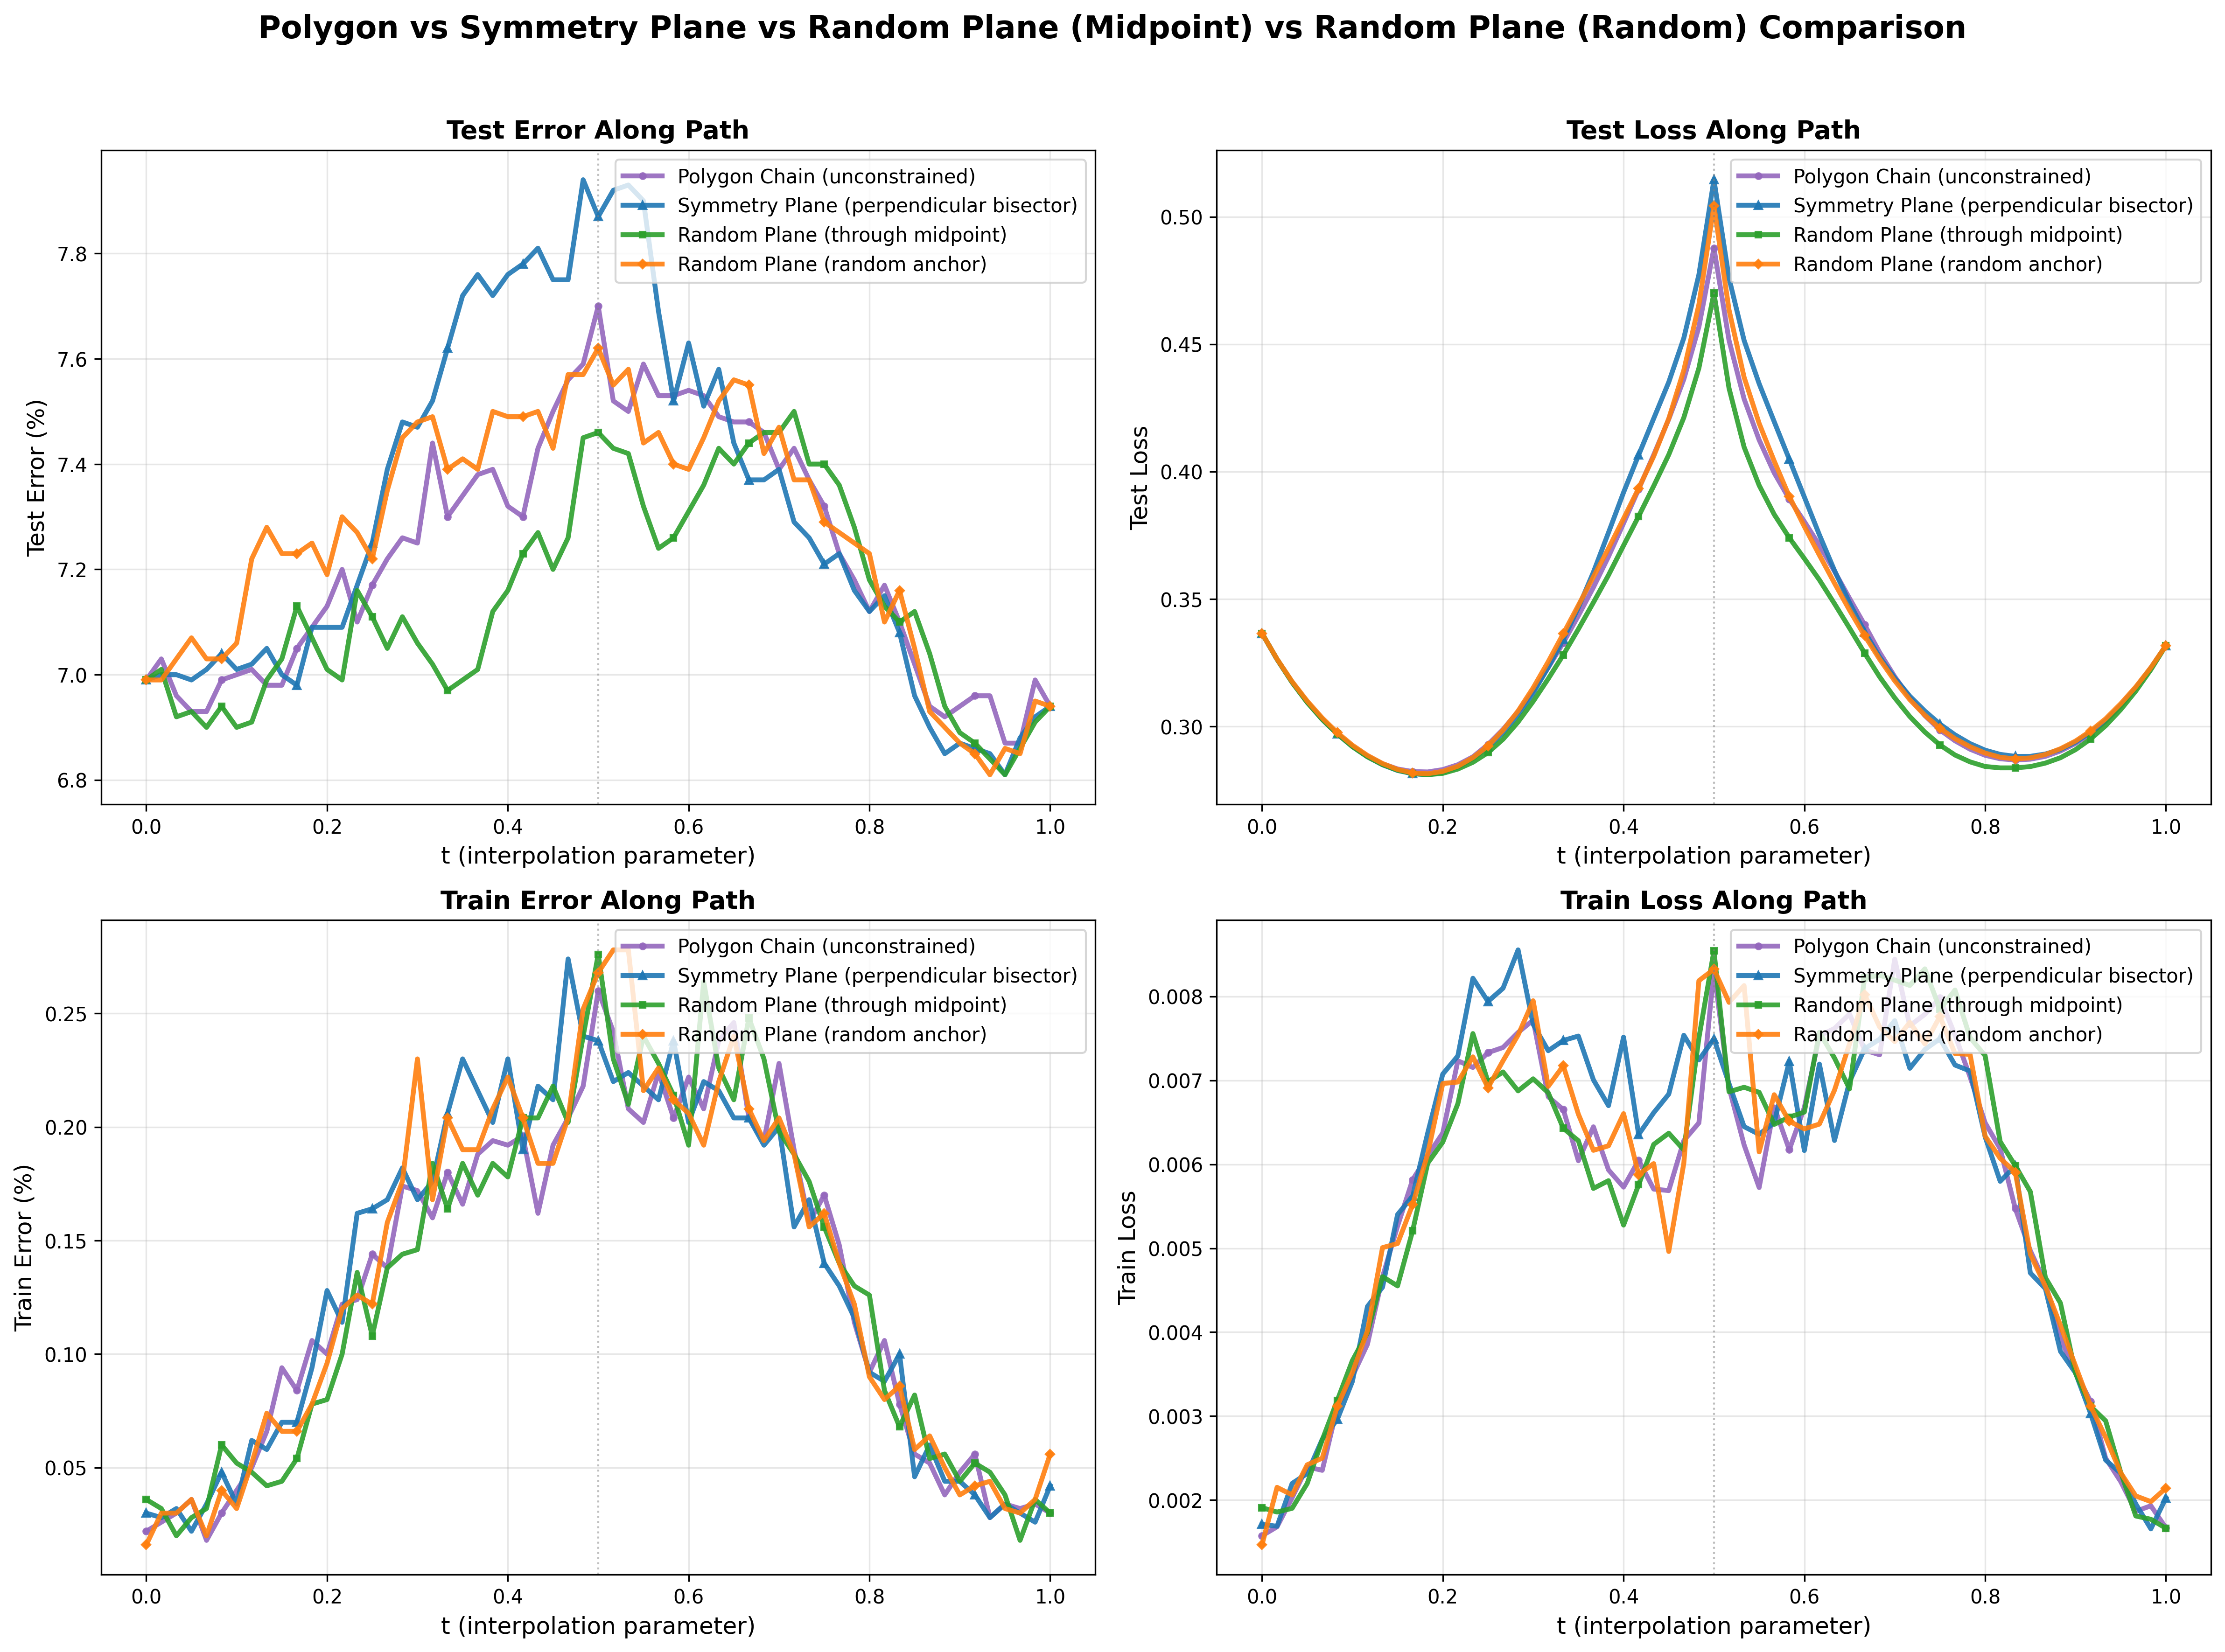
\includegraphics[width=0.8\linewidth]{random_planes_comp.png}
    \label{fig:placeholder}
\end{figure}



\begin{table}[h]
\centering
\caption{Hyperplane Constraint Configurations}
\begin{tabular}{lll}
\hline
\textbf{Plane Type} & \textbf{Anchor Point} & \textbf{Normal Vector} \\
\hline
Symmetry Plane & Midpoint $(w_0+w_1)/2$ & $w_1-w_0$ \\
Random Plane (Midpoint) & Midpoint $(w_0+w_1)/2$ & Random unit vector \\
Random Plane (Random) & Random $\alpha w_0+(1-\alpha)w_1$ & Random unit vector \\
\hline
\end{tabular}
\end{table}

\textbf{Results:} All three hyperplane constraints yielded nearly identical connectivity performance. Test error curves, training loss patterns, and barrier heights showed no meaningful differences between symmetry plane, random plane through midpoint, and totally random plane configurations. The unconstrained polygon chain also produced similar results.

\textbf{Explanation:} This surprising robustness arises from the extremely weak nature of the constraint. Removing a single direction from $\sim$15 million dimensional parameter space (reducing from $N$ to $N-1$ dimensions) has negligible impact on the optimization landscape. The loss surface is sufficiently rich that excellent low-loss paths exist within any $(N-1)$-dimensional hyperplane, regardless of which single direction is removed or where the anchor point is placed. Mode connectivity is robust enough that the specific geometric properties of the symmetry plane provide no advantage over arbitrary hyperplane constraints.

This result suggests that prior findings showing symmetry plane constraints maintain connectivity are not due to special geometric properties of the perpendicular bisector, but rather because any hyperplane constraint in such high-dimensional spaces is effectively non-restrictive.

\subsection{Middle Bend Initialization Strategies}

To investigate sensitivity to initial conditions, we compared different strategies for initializing the trainable middle bend in B\'{e}zier curves. Three initialization methods were tested: (1) biased linear interpolation, (2) perturbed midpoint with Gaussian noise, and (3) sphere-constrained initialization. No regularization was used here.

\textbf{Biased Linear Initialization:} Middle bend initialized as $\theta_{\text{init}} = \alpha w_0 + (1-\alpha) w_1$ with $\alpha \in \{0.75, 0.9\}$, positioning the initial point closer to one endpoint rather than the geometric midpoint ($\alpha = 0.5$).

\begin{figure}
    \centering
    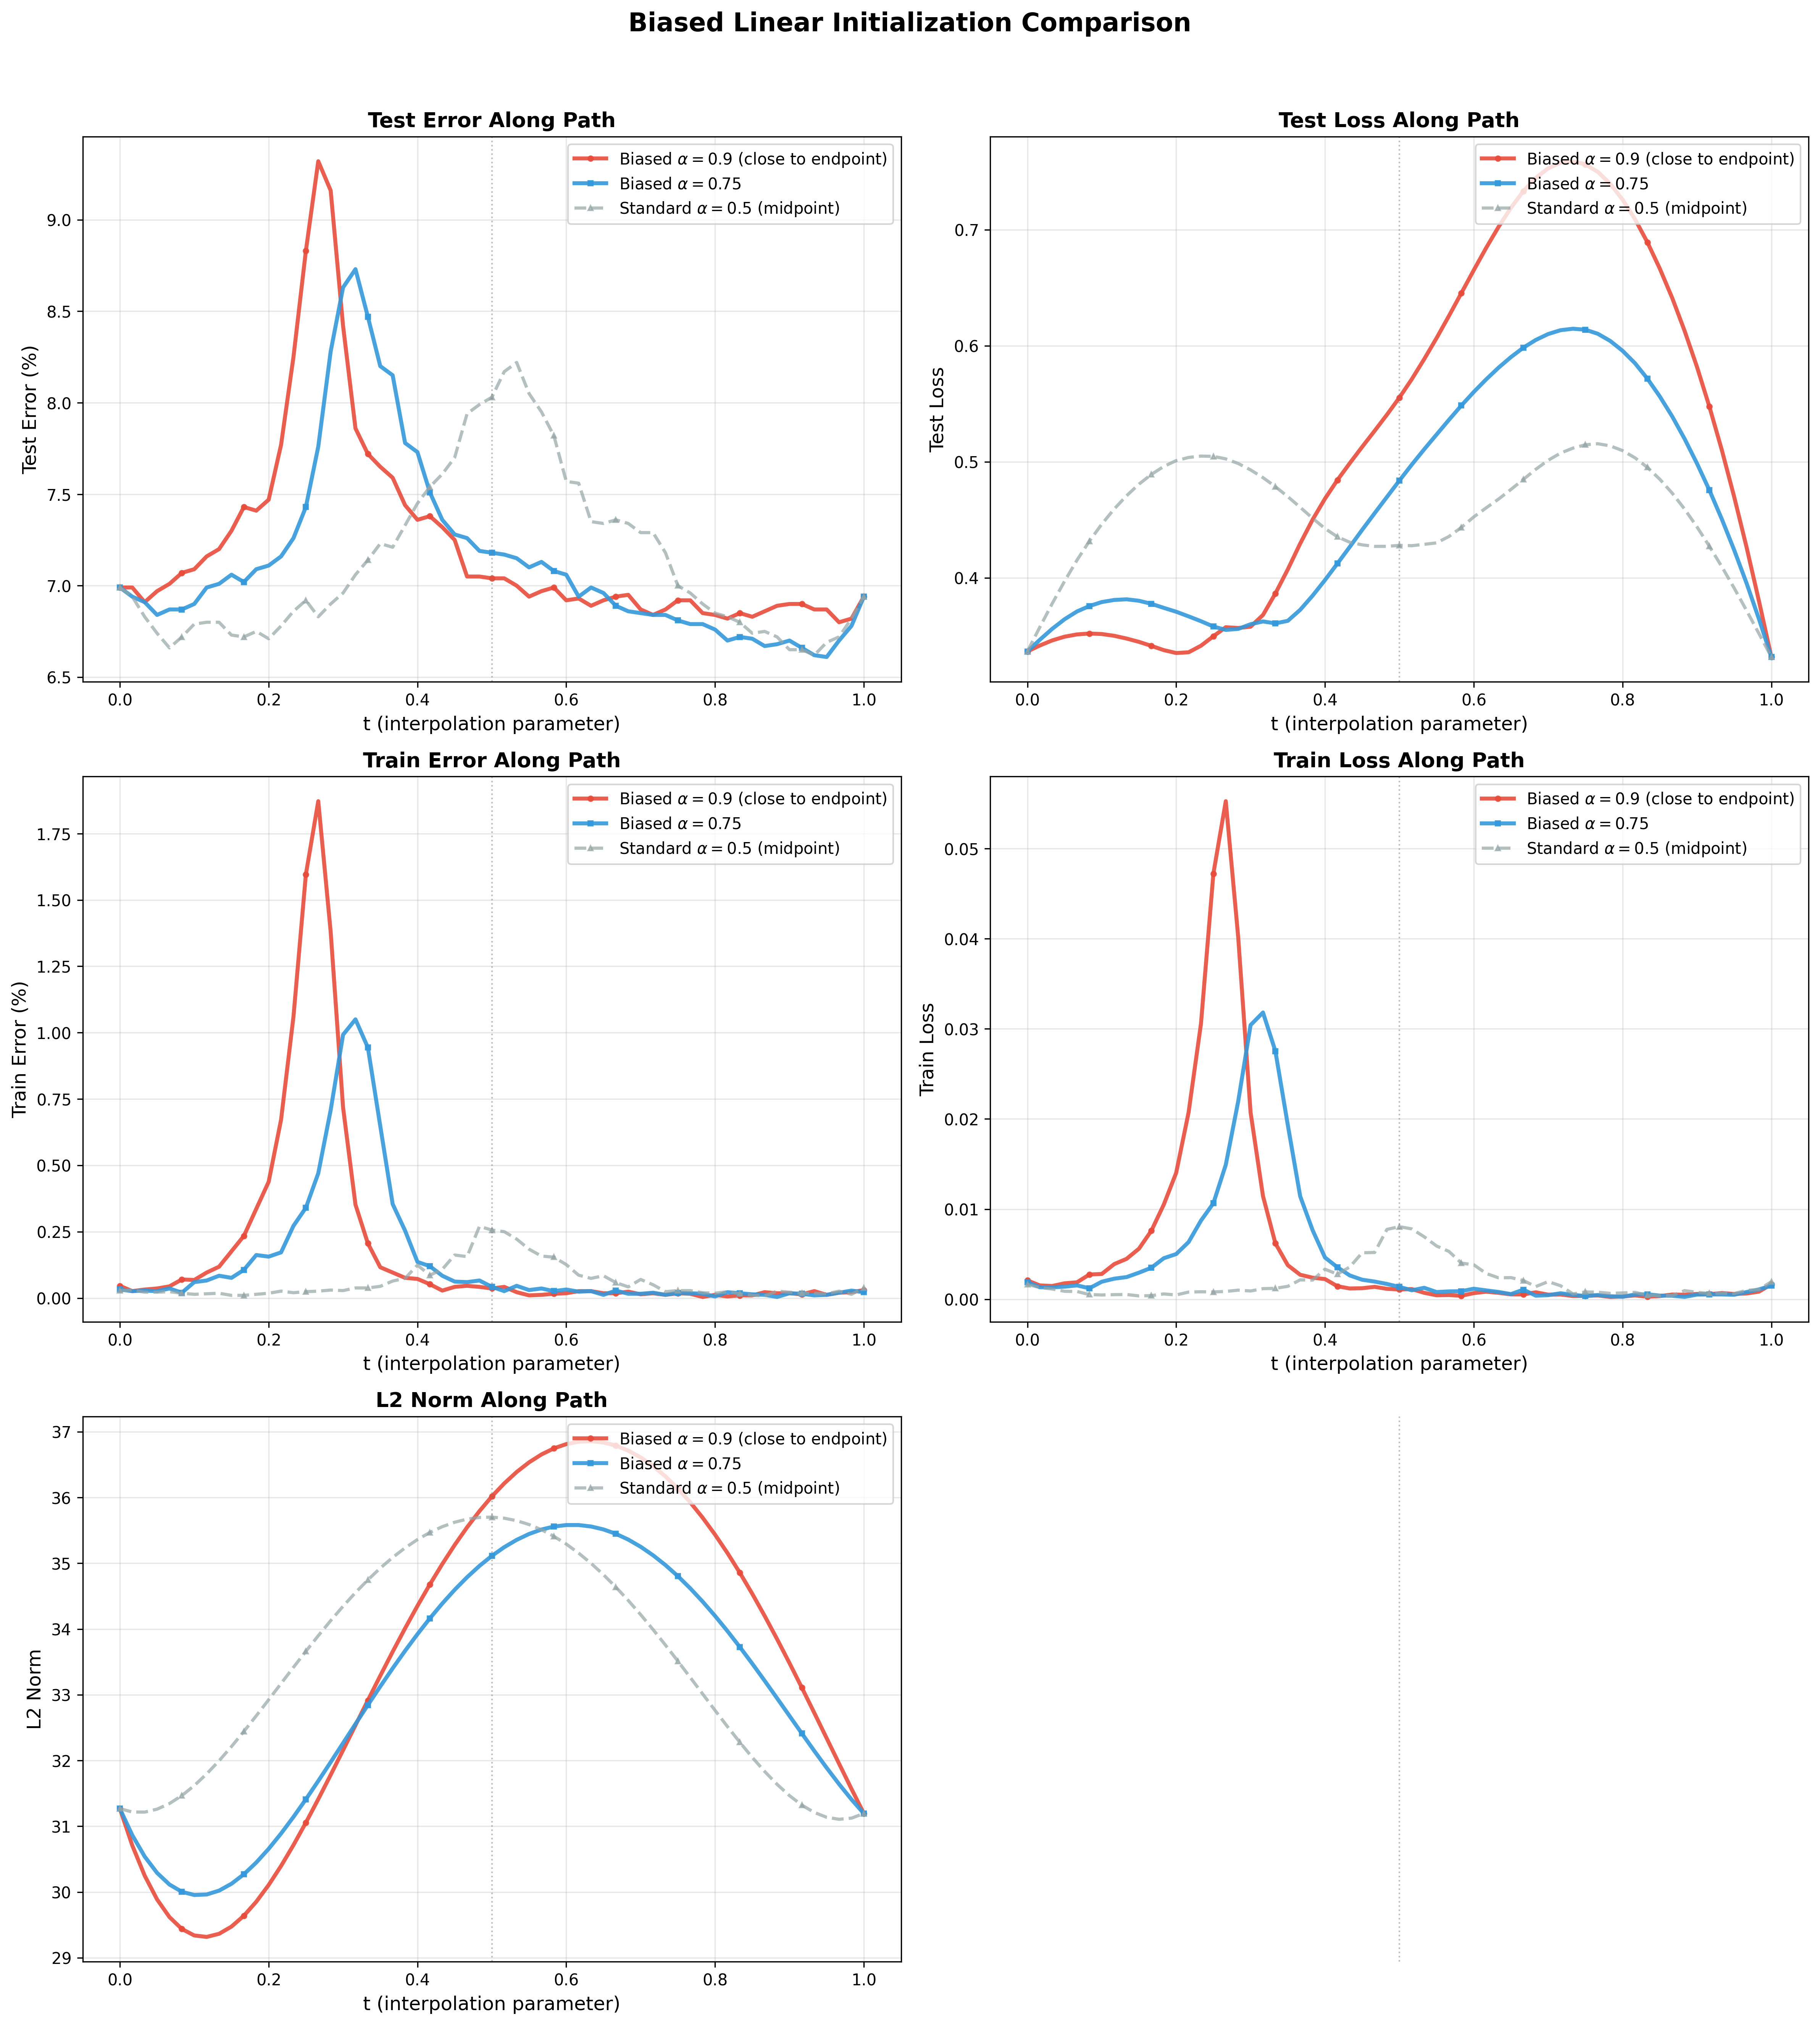
\includegraphics[width=1\linewidth]{init_comparison.png}
    \label{fig:placeholder}
\end{figure}

\begin{figure}
    \centering
    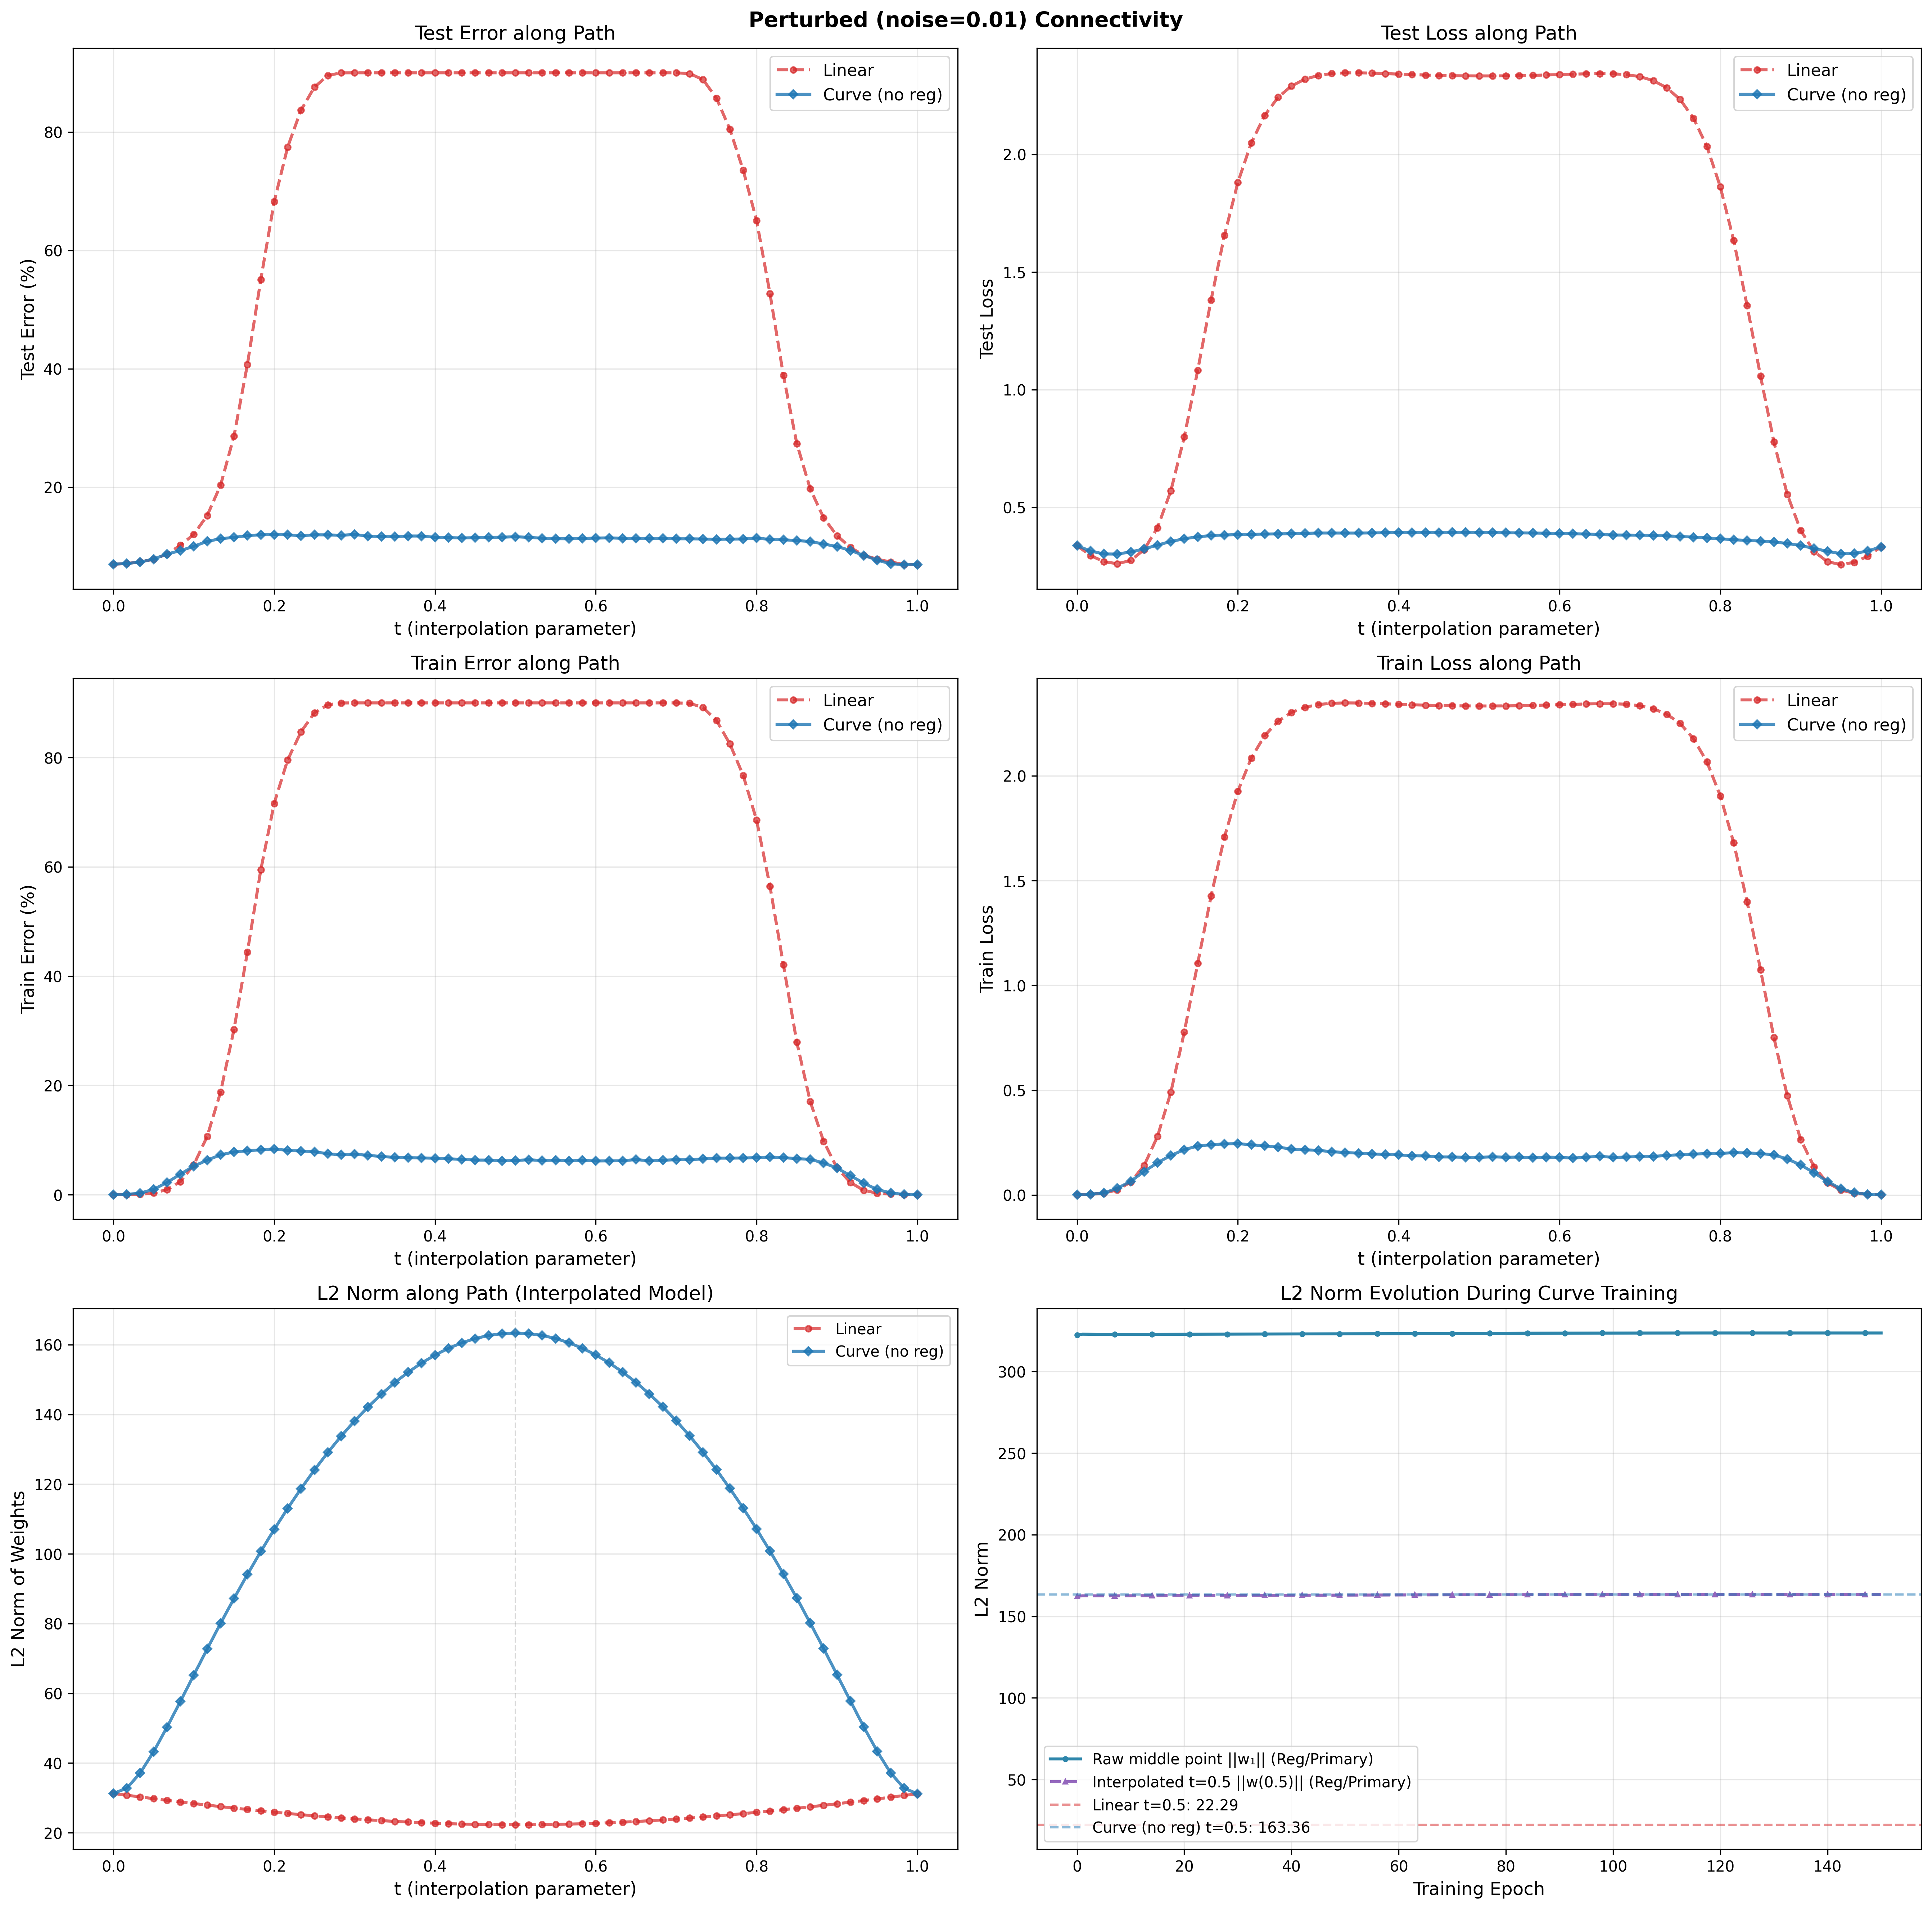
\includegraphics[width=1\linewidth]{perturbed.png}
    \label{fig:placeholder}
\end{figure}

\textbf{Perturbed Initialization:} Middle bend initialized as $\theta_{\text{init}} = 0.5(w_0 + w_1) + \epsilon$ where $\epsilon \sim \mathcal{N}(0, \sigma^2 I)$ with noise scales $\sigma \in \{0.01\}$, adding random Gaussian perturbations to the standard midpoint initialization.

\textbf{Sphere-Constrained Initialization:} Middle bend initialized at the midpoint with added Gaussian noise, then projected onto a sphere centered at the midpoint. The projection targets either inside (0.9×L2 norm) or outside (1.1×L2 norm) the sphere defined by the linear interpolation path.

\textbf{Results:} For biased linear initialization, all initialization strategies converged to low-loss paths; however, the barrier height increased with distance from the midpoint. Perturbed initialization with Gaussian noise also managed to find a decent low-loss path. Because of no regularization, there was no incentive to decrease L2 norm, and therefore the trained bend-point of the B\'{e}zier curve remained at the initialized distance from the origin (around 320, which is high in comparison with 40 for regularized standard midpoint training). Sphere-constrained initialization with added noise produced a curve very similar to normal midpoint initialization, so no plots were attached.

\textbf{Interpretation:} The robustness to initialization strategy indicates that the mode connectivity optimization problem has favorable geometric properties. The loss surface does not exhibit narrow basins or strong dependence on precise initial positioning, suggesting that successful path-finding is a robust property of the underlying optimization landscape rather than a consequence of carefully tuned initialization. This supports the hypothesis that low-loss paths between modes are abundant rather than rare in the high-dimensional parameter space.

\subsection{ConvFC on Fashion-MNIST}

To validate our findings across different architectures and datasets, we conducted the same connectivity experiments using a ConvFC architecture on Fashion-MNIST. The results were qualitatively similar to VGG16 on CIFAR-10, demonstrating that mode connectivity phenomena generalize across model architectures and tasks.

\textbf{Key Observations:} The connectivity behavior between independently trained models (seed0-seed1) showed similar low-loss path characteristics as in the VGG16/CIFAR-10 configuration. However, one notable difference emerged: the L2 norm along the trained curve path exhibited asymmetry around $t=0.5$, unlike the more symmetric behavior observed in VGG16. Interestingly, despite this L2 asymmetry, the linear interpolation barrier remained perfectly symmetric around $t=0.5$. Moreover, the barriers are visibly thinner than in the case of VGG16 on CIFAR-10.
\begin{figure}[H]
    \centering
    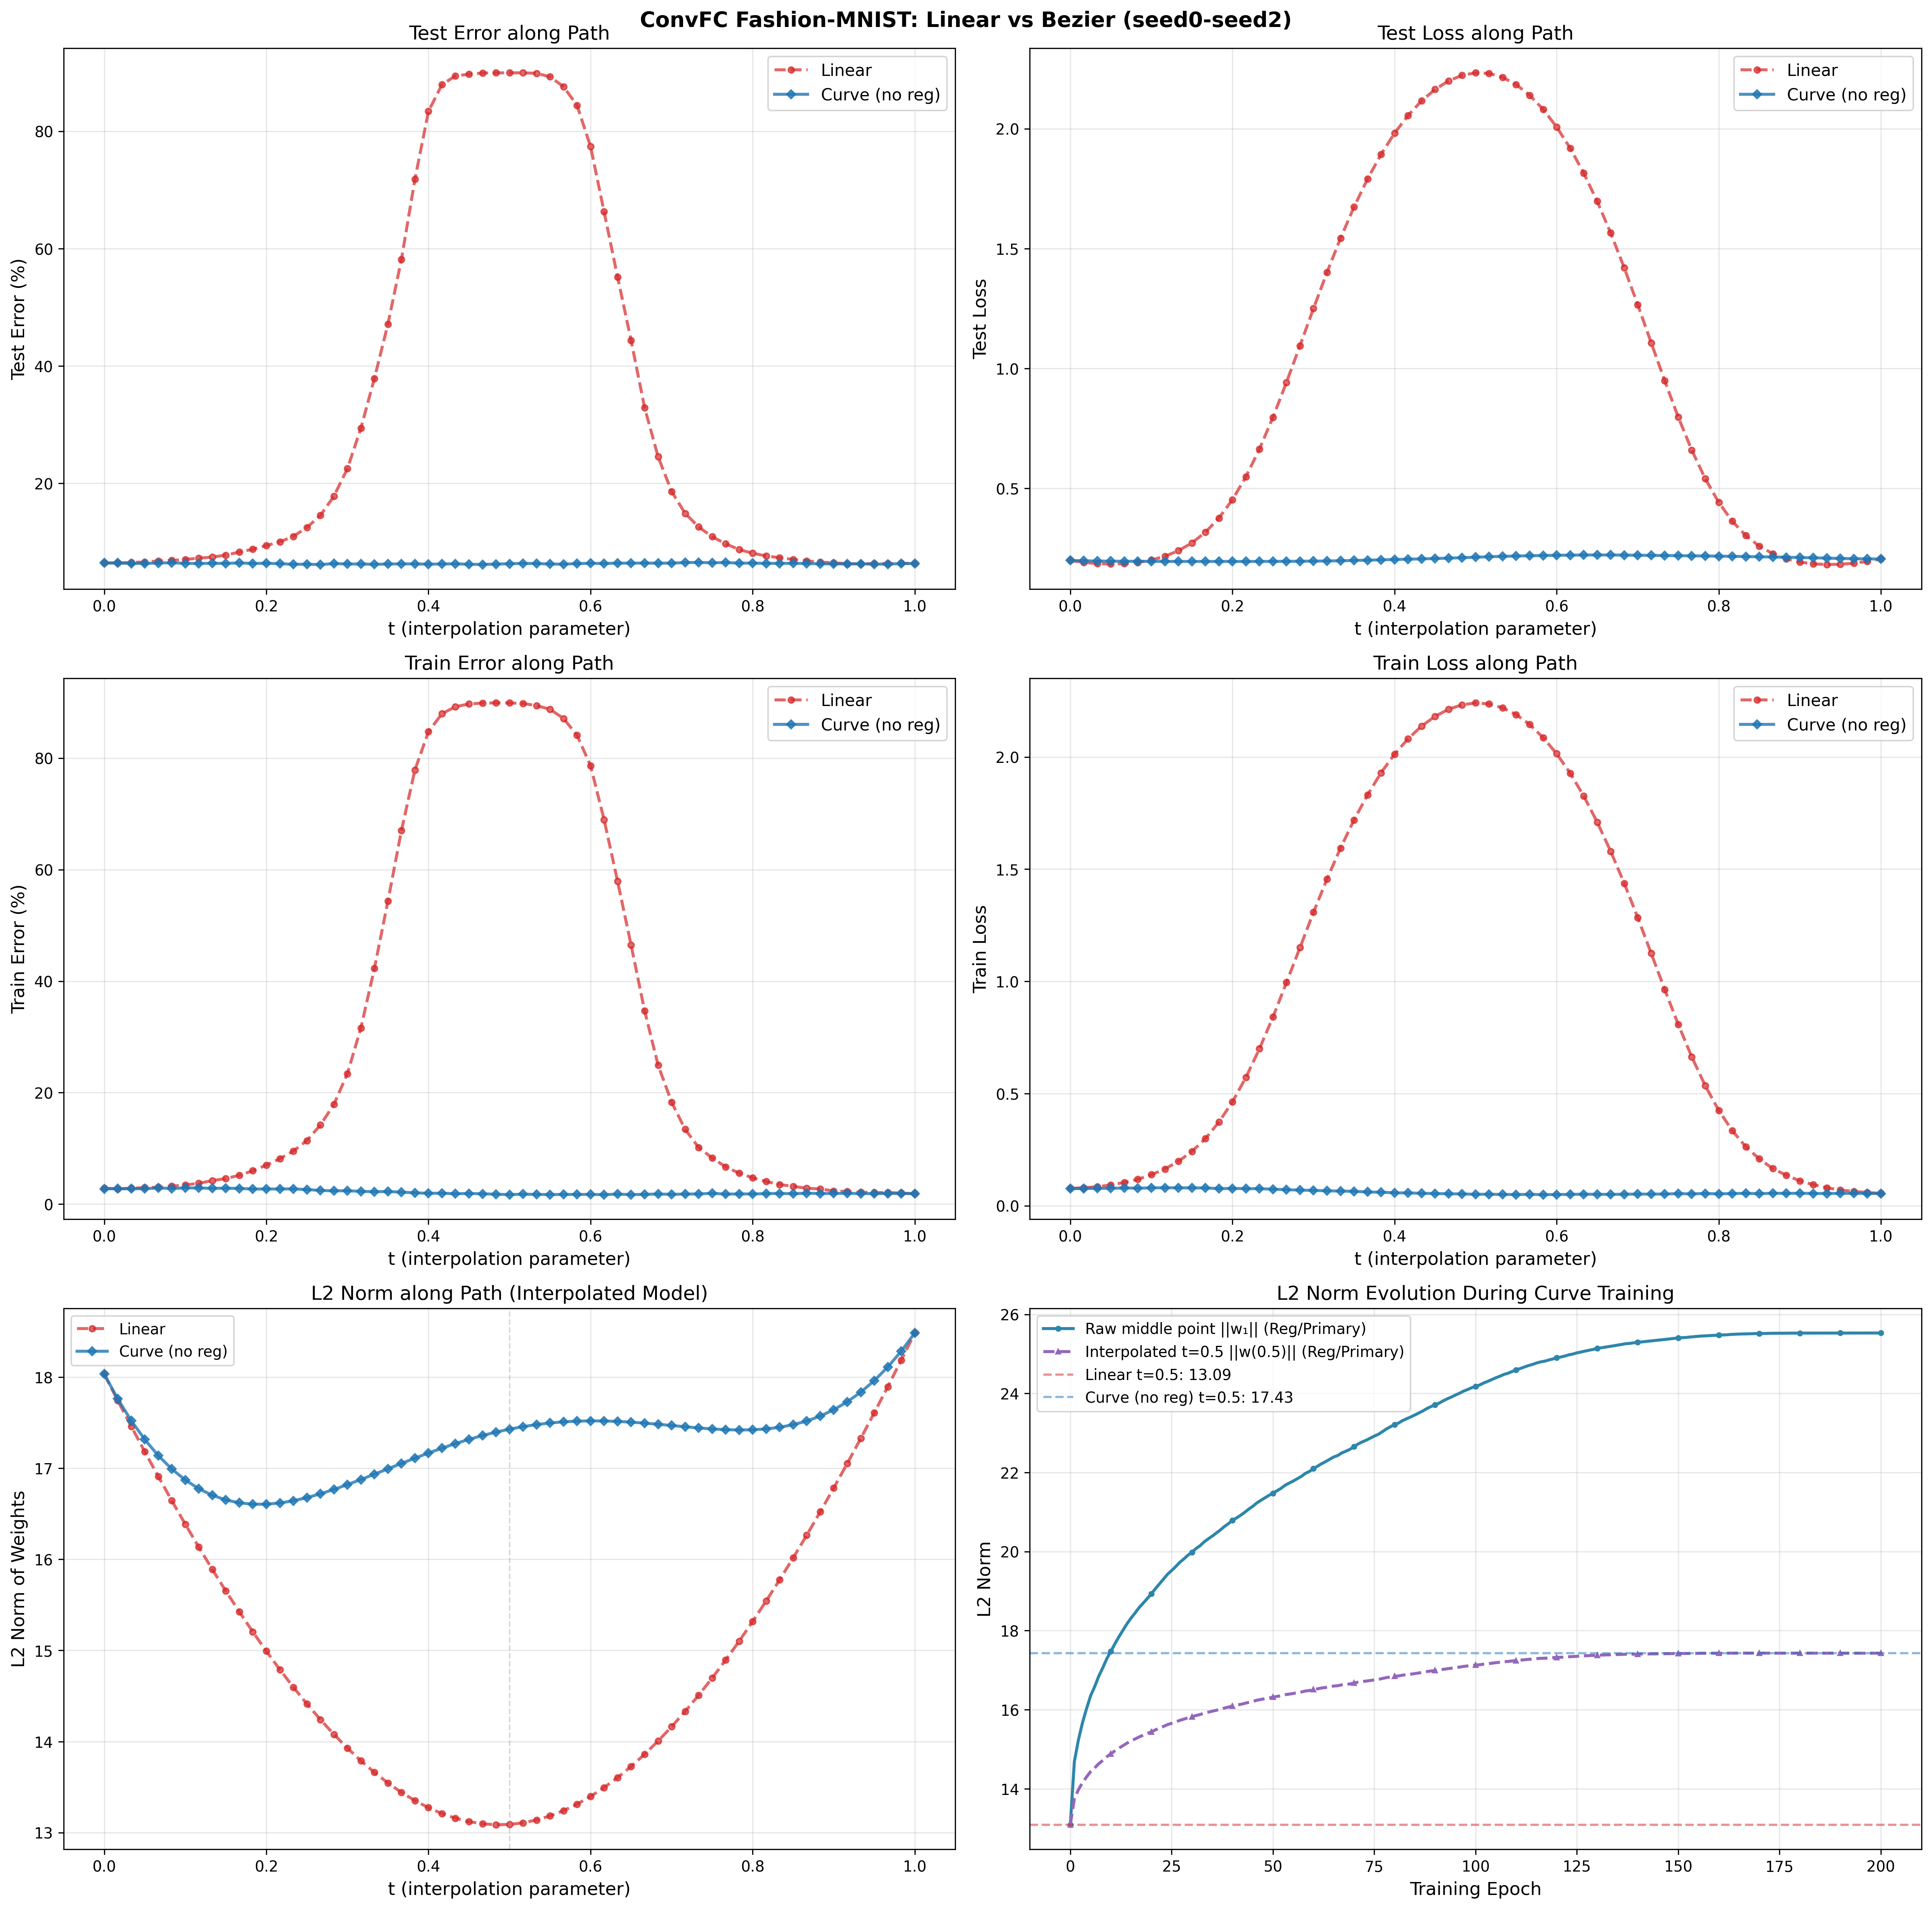
\includegraphics[width=0.9\linewidth]{convfc_example.png}
\end{figure}
\newpage

\begin{figure}
    \centering
    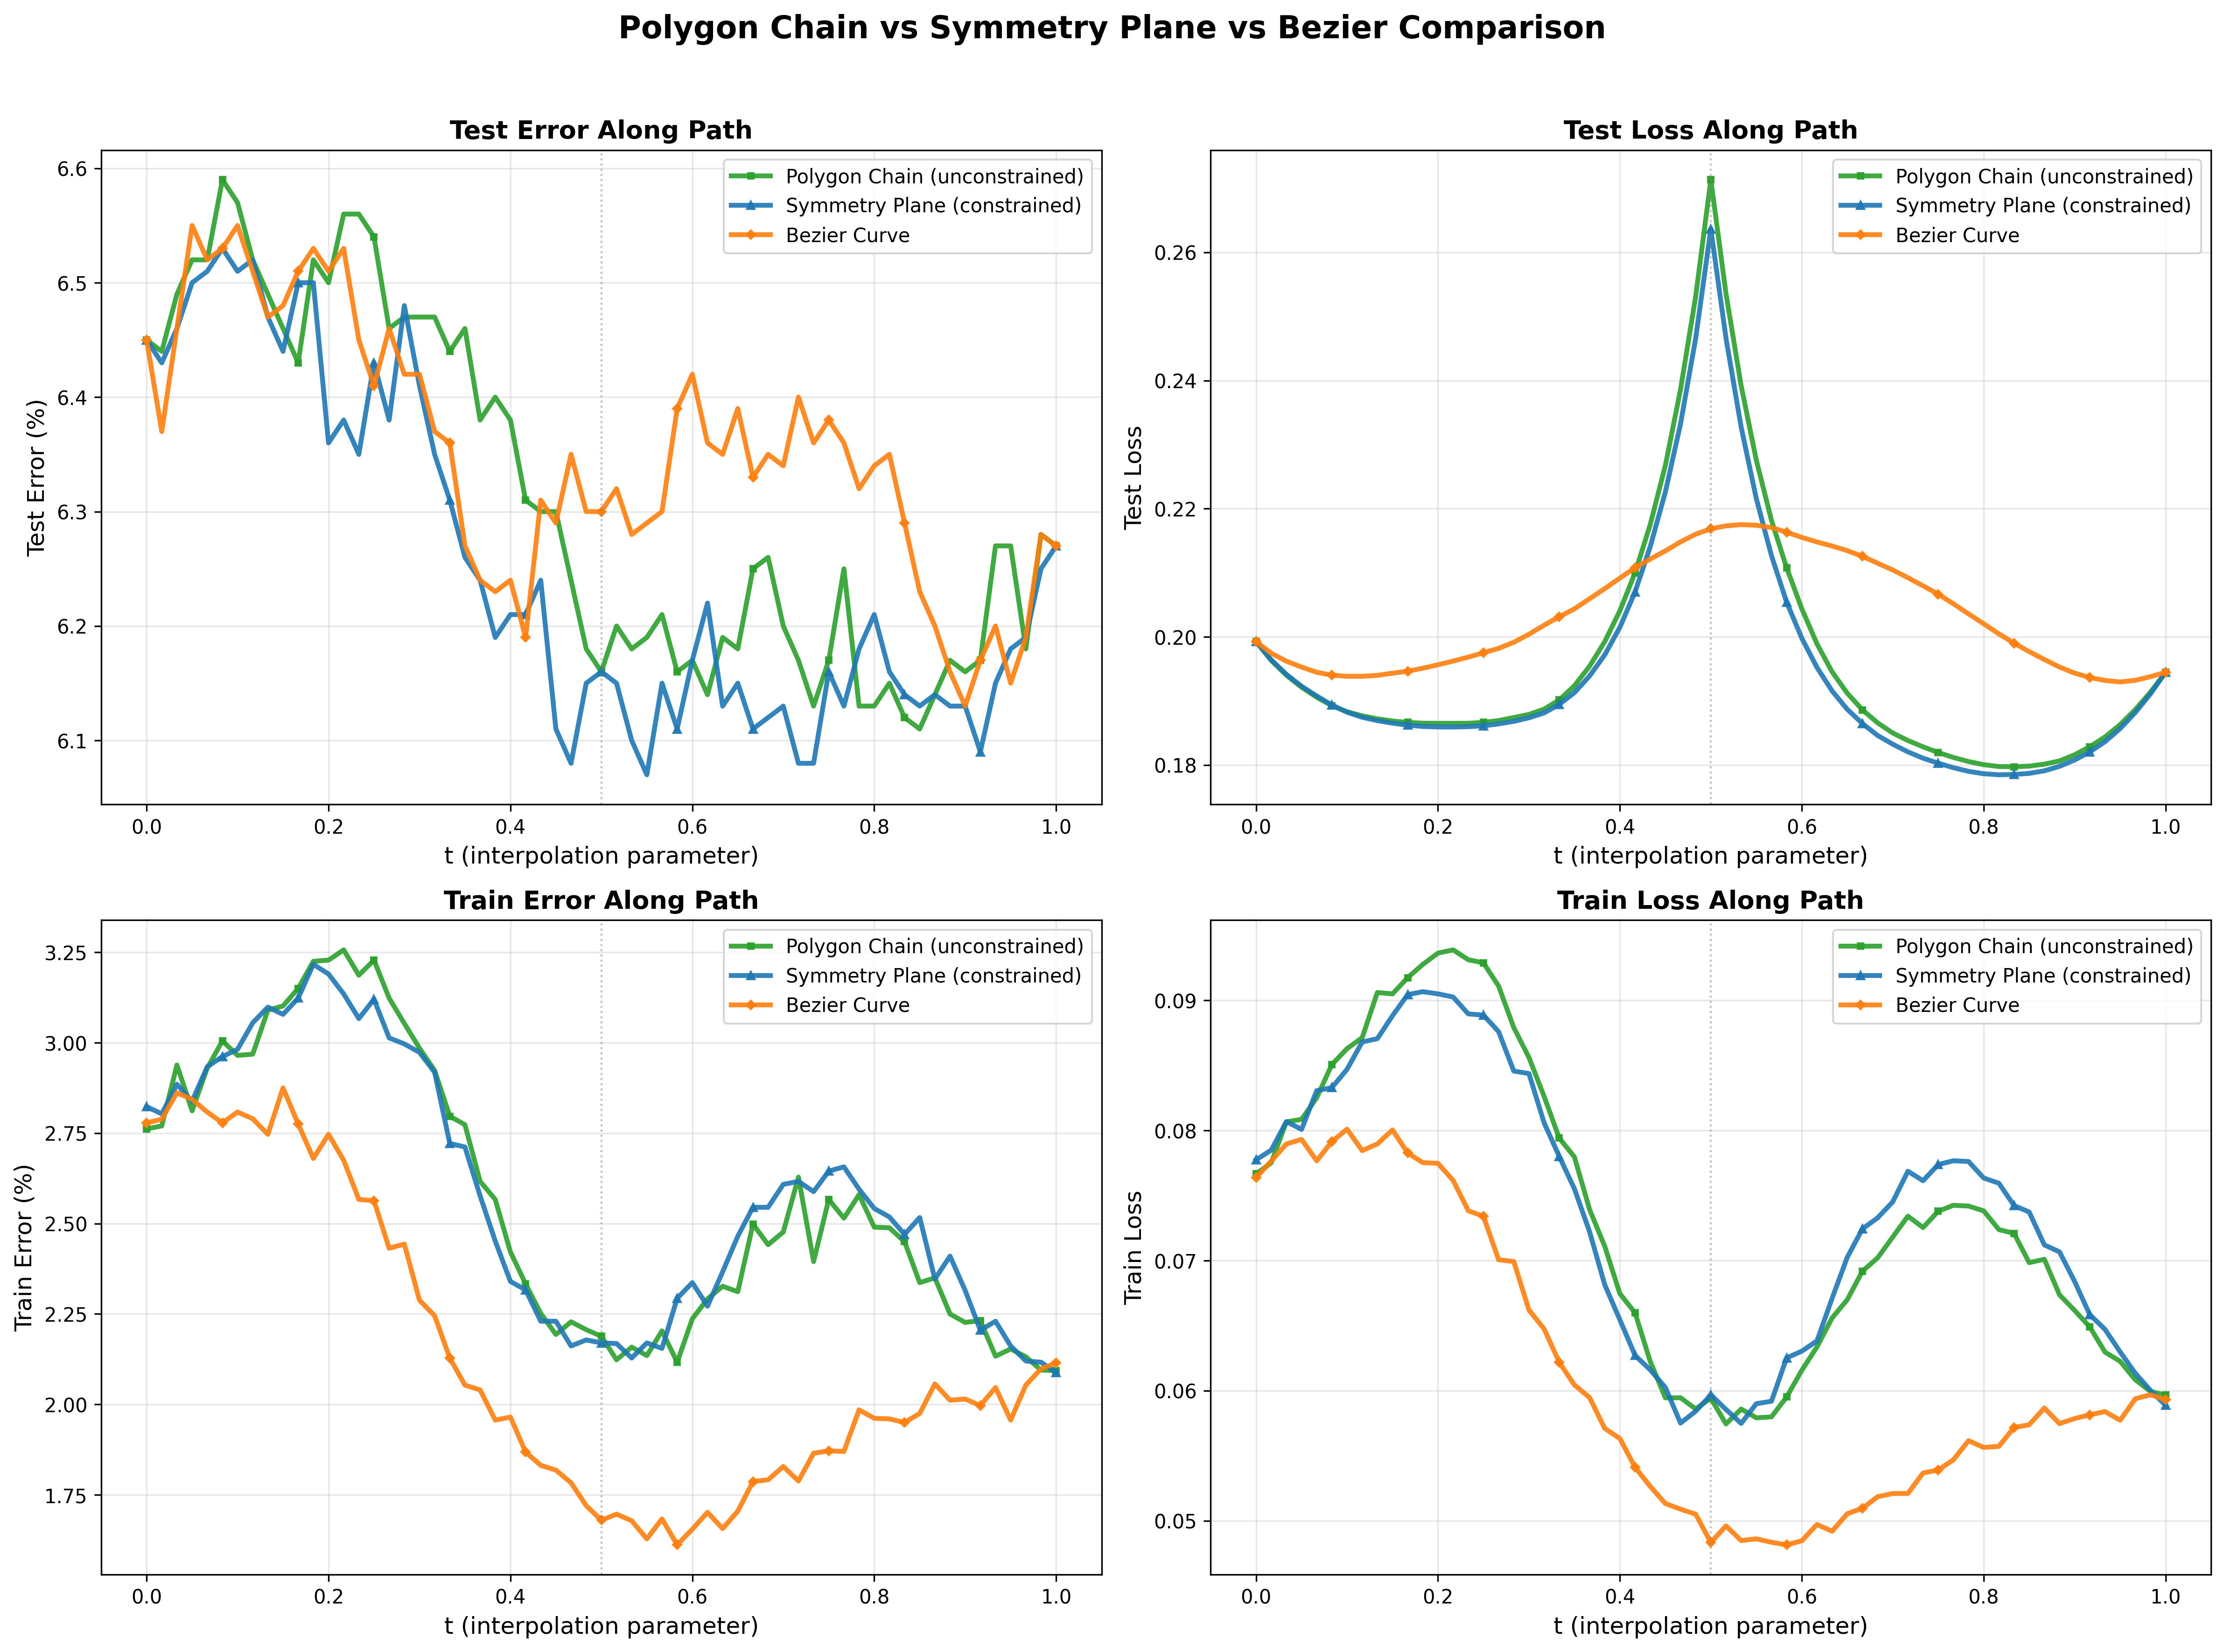
\includegraphics[width=0.75\linewidth]{seed0seed1curve_comparison.png}
    \caption{Seed0-Seed1 low-loss path finding methods comparison}
\end{figure}

\textbf{Interpretation:} The asymmetric L2 norm profile suggests that the optimization has found a path that deviates more strongly in one direction from the linear interpolation. This demonstrates that multiple geometric paths through parameter space can achieve similar loss profiles, further supporting the abundance of low-loss connectivity paths in high-dimensional loss landscapes.

\subsection{Observations on Loss Curve Characteristics}

Through detailed code analysis and verification experiments, several important observations emerged regarding the loss and accuracy curves along connectivity paths:

\textbf{Curve Smoothness:} Under standard evaluation conditions (without random augmentations), the loss curves exhibit very smooth, continuous behavior. Initial apparent noise in some curves was traced to random data augmentations (horizontal flips, random crops) being inadvertently applied during evaluation on the training split. This was corrected to ensure consistent evaluation conditions.

\textbf{Train vs.\ Test Loss Differences:} The apparent differences between train and test loss curves are correct and expected. In both VGG16 on CIFAR-10 and ConvFC on Fashion-MNIST, the models exhibited overfitting on the training data. Consequently, the train loss curves appear nearly flat along the connectivity path when plotted on the same scale as test loss curves. This does not indicate different data distributions or evaluation errors---rather, it reflects the models' strong memorization of the training set. The test loss curves, evaluating on unseen data, naturally show higher values and more pronounced variation along the path.

\textbf{Endpoint Consistency:} Initial observations showed that loss and accuracy values at the endpoints ($t=0$ and $t=1.0$) varied slightly across different path-finding methods. This variation was also attributed to random augmentations being applied during batch normalization statistics updates on the training split. When augmentations were disabled for evaluation, endpoint values became consistent across all methods, as expected.

\textbf{Conclusion:} The distinct visual characteristics of train versus test loss plots are correct and informative. They reveal the degree of overfitting in the models and demonstrate that the connectivity phenomena exist in the generalization regime (test data), not merely as artifacts of training set memorization. Future experiments will ensure that data augmentations are disabled during all evaluation procedures to maintain consistency and interpretability of results.
The trained path at t=0.5 has learned to:

Better fit the training data (train loss goes down)
At the cost of generalization (test loss goes up)




\section{References}
\begin{itemize}
    \item Draxler et al.\ (2018): Essentially No Barriers in Neural Network Energy Landscape.
    \item Freeman \& Bruna (2017): Topology and Geometry of Half-Rectified Network Optimization.
    \item Entezari et al.\ (2021): The Role of Permutation Invariance in Linear Mode Connectivity of Neural Networks.
    \item Ainsworth et al.\ (2023): Git Re-Basin: Merging Models Modulo Permutation Symmetries.
    \item Zhan et al.\ (2025): Analyzing the Role of Permutation Invariance in Linear Mode Connectivity.
    \item Crisostomi et al.\ (2024): Cycle-Consistent Multi-Model Merging (C$^2$M$^3$).
\end{itemize}

\end{document}